\documentclass[12pt]{article}
\usepackage{amsmath}
\usepackage{graphicx}
\usepackage{hyperref}
\usepackage{listings}
\usepackage{color}

\title{Operating System Course Report - First Half of the Semester}
\author{A class}
\date{\today}

\begin{document}
	
	\maketitle
	\newpage
	
	\tableofcontents
	\newpage
	
	\section{Introduction}
	This report summarizes the topics covered during the first half of the Operating System course. It includes theoretical concepts, practical implementations, and assignments. The course focuses on the fundamentals of operating systems, including system architecture, process management, CPU scheduling, and deadlock handling.
	
	\section{Course Overview}
	\subsection{Objectives}
	The main objectives of this course are:
	\begin{itemize}
		\item To understand the basic components and architecture of a computer system.
		\item To learn process management, scheduling, and inter-process communication.
		\item To explore file systems, input/output management, and virtualization.
		\item To study the prevention and handling of deadlocks in operating systems.
	\end{itemize}
	
	\subsection{Course Structure}
	The course is divided into two halves. This report focuses on the first half, which covers:
	\begin{itemize}
		\item Basic Concepts and Components of Computer Systems
		\item System Performance and Metrics
		\item System Architecture of Computer Systems
		\item Process Description and Control
		\item Scheduling Algorithms
		\item Process Creation and Termination
		\item Introduction to Threads
		\item File Systems
		\item Input and Output Management
		\item Deadlock Introduction and Prevention
		\item User Interface Management
		\item Virtualization in Operating Systems
	\end{itemize}
	
	\section{Topics Covered}
	
	\subsection{Basic Concepts and Components of Computer Systems}
	This section explains the fundamental components that make up a computer system, including the CPU, memory, storage, and input/output devices.
	
	\subsection{System Performance and Metrics}
	This section introduces various system performance metrics used to measure the efficiency of a computer system, including throughput, response time, and utilization.
	
	\subsection{System Architecture of Computer Systems}
	Describes the architecture of modern computer systems, focusing on the interaction between hardware and the operating system.
	
	\subsection{Process Description and Control}
	Processes are a central concept in operating systems. This section covers:
	\begin{itemize}
		\item Process states and state transitions
		\item Process control block (PCB)
		\item Context switching
	\end{itemize}
	
	\subsection{Scheduling Algorithms}
	This section covers:
	\begin{itemize}
		\item First-Come, First-Served (FCFS)
		\item Shortest Job Next (SJN)
		\item Round Robin (RR)
	\end{itemize}
	It explains how these algorithms are used to allocate CPU time to processes.
	
	\subsection{Process Creation and Termination}
	Details how processes are created and terminated by the operating system, including:
	\begin{itemize}
		\item Process spawning
		\item Process termination conditions
	\end{itemize}
	
	\subsection{Introduction to Threads}
	This section introduces the concept of threads and their relation to processes, covering:
	\begin{itemize}
		\item Single-threaded vs. multi-threaded processes
		\item Benefits of multithreading
	\end{itemize}
	
	\subsection{File Systems}
	File systems provide a way for the operating system to store, retrieve, and manage data. This section explains:
	\begin{itemize}
		\item File System Concepts
		\item File attributes
		\item Operations on files
		\item File types
		\item File structure
		\item File access methods
		\item Directory structure
		\\Direktori adalah kumpulan titik yang berisi informasi tentang semua file. Beberapa sistem menyimpan ratusan file pada disk ratusan \textit{gigabyte}. Untuk mengatur semua data menggunakan organisasi yang dilakukan dalam dua bagian.
		
		\begin{figure}[h!]
			\centering
			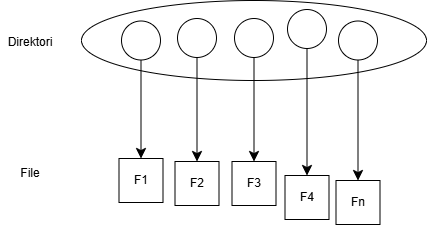
\includegraphics[width=0.8\textwidth]{aset/Halaman-1.drawio.png}
			
		\end{figure}
		\\Pertama, system file dipecah ke dalam partisi, yang disebut juga “\textit{minidisc}” (pada mesin IBM) atau “volume” (pada mesin PC dan \textit{Macintosh}). Setiap disk pada sistem berisi sedikitnya satu partisi, merupakan struktur \textit{low-level} dimana file dan direktori berada. Terkadang, partisi digunakan untuk menentukan beberapa daerah terpisah dalam satu disk, yang diperlakukan sebagai perangkat penyimpan yang terpisah. Sistem lain menggunakan partisi yang lebih besar dari sebuah disk untuk mengelompokkan disk ke dalam satu struktur logika. Kedua, setiap partisi berisi informasi mengenai file di dalamnya. Informasi ini disimpan pada\textit{ entry }dalam “\textit{device directory atau volume table of contents}”. Perangkat direktori (atau direktori) menyimpan informasi seperi nama, lokasi, ukuran dan tipe untuk semua file dari partisi tersebut. Organisasi file yang umum dapat dilihat pada gambar .
		\begin{figure}[h!]
			\centering
			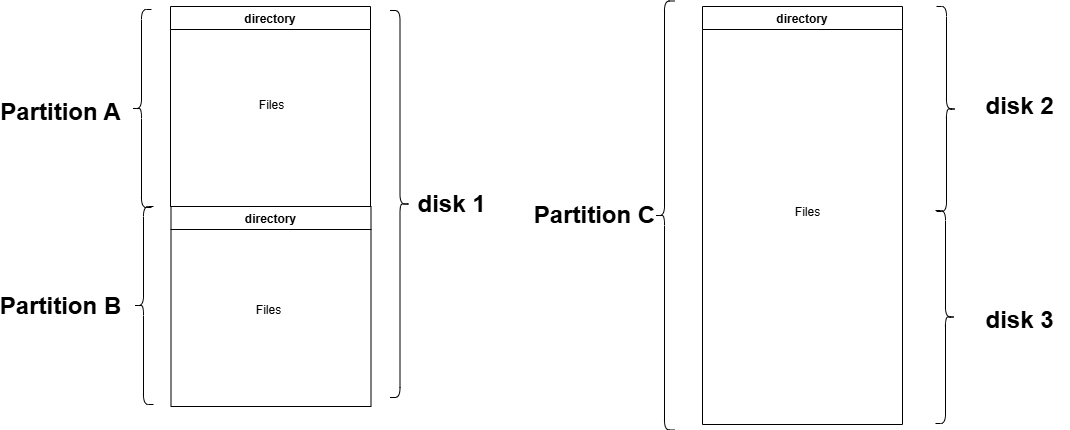
\includegraphics[width=0.8\textwidth]{aset/Halaman-2.drawio.png}
			
		\end{figure}
		\\ Informasi yang terdapat pada direktori adalah :  Nama, Tipe, Alamat, Panjang saat ini,  Panjang maksimum, Tanggal akses terakhir, Tanggal perubahan terakhir, ID pemilik, Informasi proteksi . Beberapa operasi yang dibentuk pada direktori adalah : Mencari file (\textit{search}),  Membuat file (\textit{create}), Menghapus file (\textit{delete}), Mendaftar suatu direktori (\textit{list}), Mengubah nama file (\textit{r\textit{ename}}),  Melintasi sistem file (\textit{traverse})   
		Organisasi file dan direktori disarankan yang seefisien mungkin sehingga dapat menempatkan file dengan cepat. Selain itu dalam penamaan file dan direktori harus nyaman untuk\textit{ user}. Dua \textit{user} dapat memberikan nama file yang sama. File yang sama dapat mempunyai beberapa nama. Dalam organisasi file dan direktori juga perlu dilakukan pengelompokan file berdasarkan \textit{property}, misalnya semua program Java, game dan lain-lain. 
		
		\subsubsection{One-level directory}
		\\Direktori ini hanya terdiri dari satu direktori untuk setiap user. Pada direktori jenis ini terjadi permasalahan penamaan dan pengelompokan berdasarkan user. 
		\begin{figure}[h!]
			\centering
			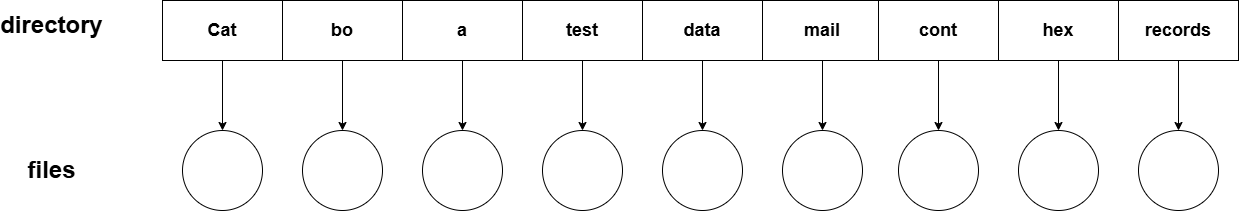
\includegraphics[width=0.8\textwidth]{aset/File system-Halaman-3.drawio.png}
			
		\end{figure}
		\subsubsection{two-level directory}
		Direktori ini terdiri dari dua level yang memisahkan direktori untuk setiap \textit{user} . Setiap file diberi nama \textit{path}, dapat mempunyai nama file yang sama untuk \textit{user} yang berbeda, mempunyai kapabilitas pencarian, tetapi belum dilakukan pengelompokan.    \begin{figure}[h!]
			\centering
			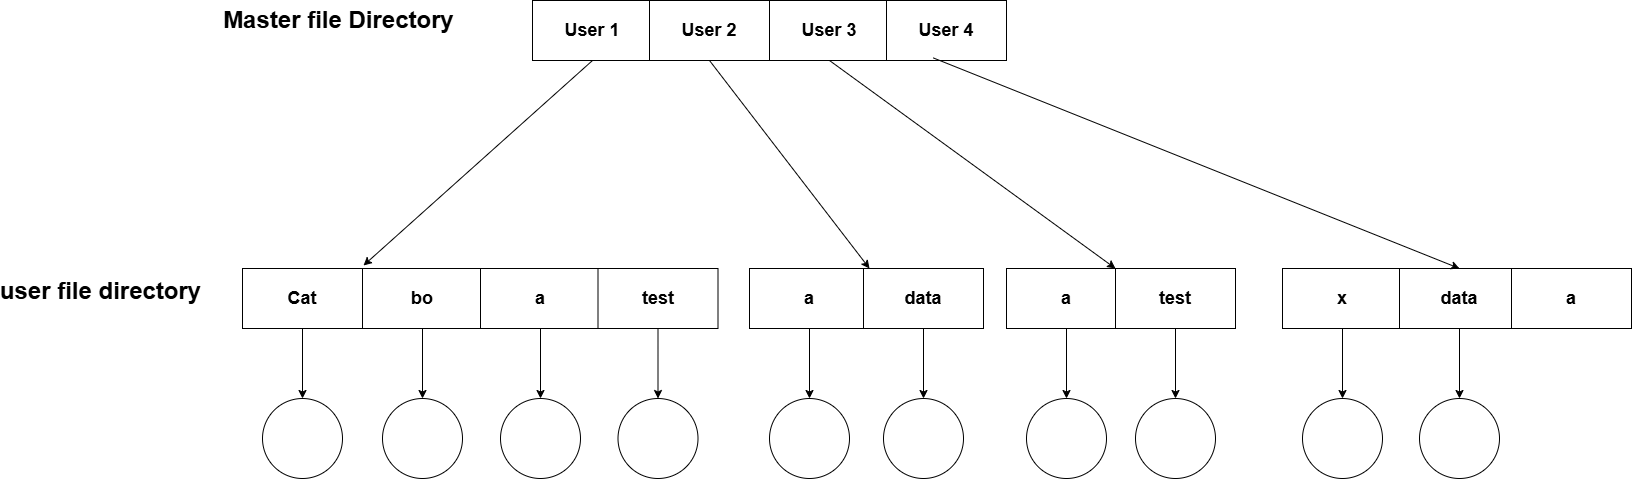
\includegraphics[width=0.8\textwidth]{aset/File system-Halaman-4.drawio.png}
			
		\end{figure}
		
		\subsubsection{Tree Structured Directory or three levels }
		Direktori berstruktur pohon merupakan struktur direktori yang biasa digunakan. Pohon mempunyai direktori \textit{root}. Setiap file pada sistem mempunyai nama \textit{path} yang unik.
		
		\begin{figure}[h!]
			\centering
			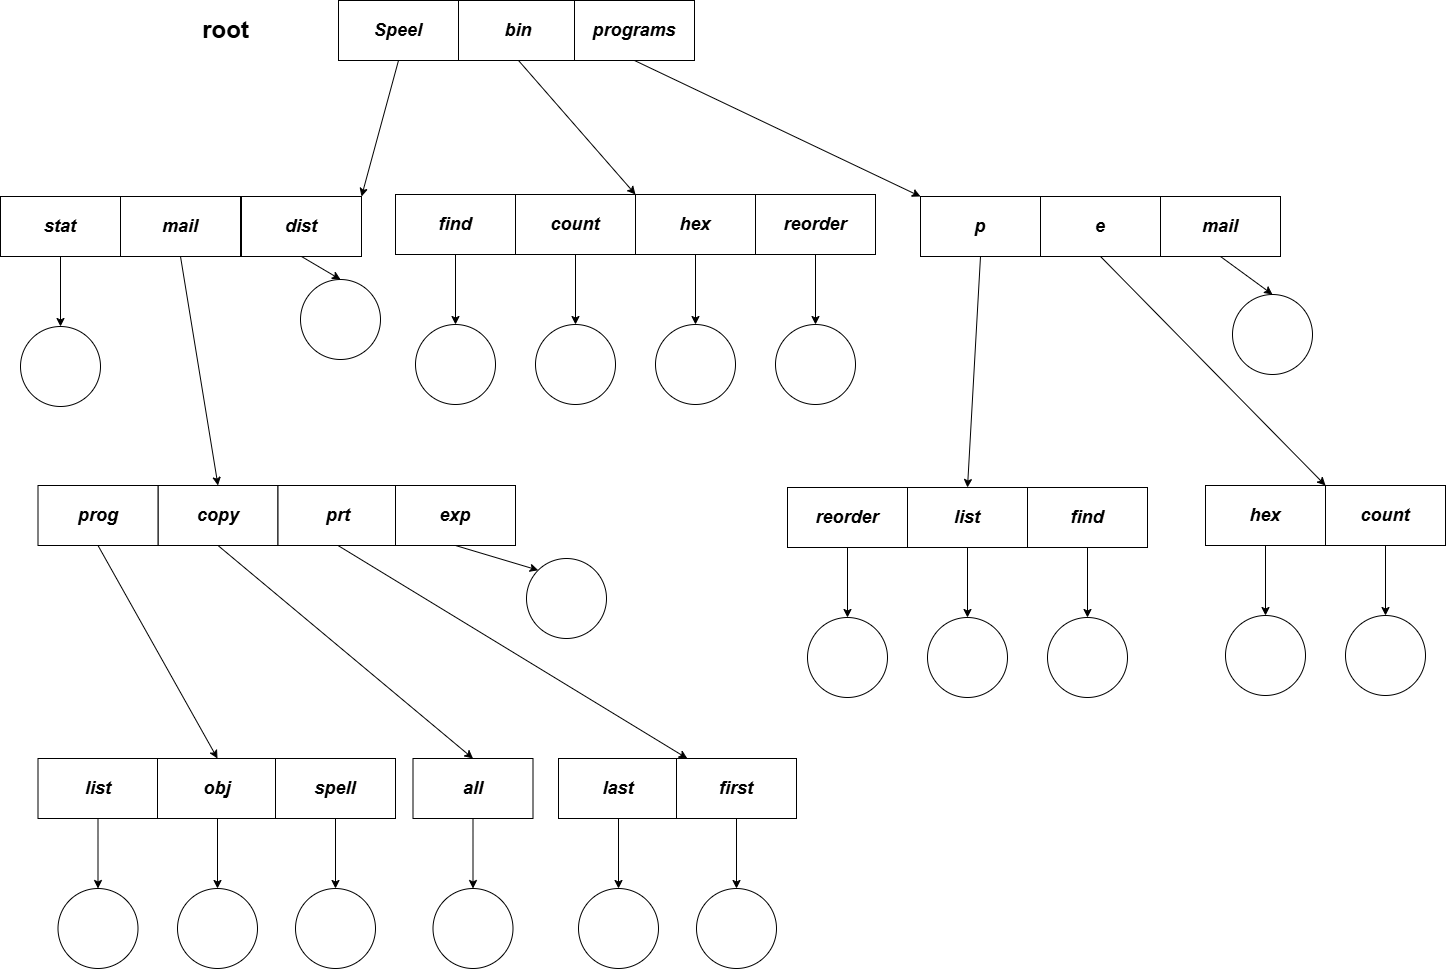
\includegraphics[width=0.5\textwidth]{aset/File system-Halaman-5.drawio.png}
			
		\end{figure}
		
		Pada direktori ini pencarian file dan direktori lebih efisien, mengelompokkan file dan dapat mengakses direktori dan sub direktori. Sebuah direktori atau subdirektori berisi kumpulan file atau sub direktori. Sebuah direktori merupakan file yang diperlakukan dengan cara khusus. Semua direktori mempunyai format internal yang sama. Satu bit dalam setiap masukan direktori merupakan masukan sebagai file (0) atau sebagai subdirektori (1). \textit{Call system} khusus digunakan untuk membuat dan menghapus direktori. Nama \textit{path} dapat dibagi menjadi dua tipe yaitu nama path “absolut” dan “relatif”. Pada saat membuat file baru akan dilakukan pada \textit{current directory}. Demikian juga pada saat membuat direktori baru.
		
		
		\item file system mounting
		\item file sharing
		\item protection
	\end{itemize}
	
	\subsection{Input and Output Management}
	Input and output management is key for handling the interaction between the system and external devices. This section includes:
	\begin{itemize}
		\item Device drivers
		\item I/O scheduling
	\end{itemize}
	
	\subsection{Deadlock Introduction and Prevention}
	Explores the concept of deadlocks and methods for preventing them:
	\begin{itemize}
		\item Deadlock conditions
		\item Deadlock prevention techniques
	\end{itemize}
	
	\subsection{User Interface Management}
	This section discusses the role of the operating system in managing the user interface. Topics covered include:
	\begin{itemize}
		\item Graphical User Interface (GUI)
		\item Command-Line Interface (CLI)
		\item Interaction between the user and the operating system
	\end{itemize}
	
	\subsection{Virtualization in Operating Systems}
	Virtualization allows multiple operating systems to run concurrently on a single physical machine. This section explores:
	\begin{itemize}
		\item Concept of virtualization
		\item Hypervisors and their types
		\item Benefits of virtualization in modern computing
	\end{itemize}
	
	\section{Assignments and Practical Work}
	\subsection{Assignment 1: Process Scheduling}
	Students were tasked with implementing various process scheduling algorithms (e.g., FCFS, SJN, and RR) and comparing their performance under different conditions.
	
	\subsection{Assignment 2: Deadlock Handling}
	In this assignment, students were asked to simulate different deadlock scenarios and explore various prevention methods.
	
	\subsection{Assignment 3: Multithreading and Amdahl's Law}
	This assignment involved designing a multithreading scenario to solve a computationally intensive problem. Students then applied **Amdahl's Law** to calculate the theoretical speedup of the program as the number of threads increased.
	
	\subsection{Assignment 4: Simple Command-Line Interface (CLI) for User Interface Management}
	Students were tasked with creating a simple **CLI** for user interface management. The CLI should support basic commands such as file manipulation (creating, listing, and deleting files), process management, and system status reporting.
	
	\subsection{Assignment 5: File System Access}
	In this assignment, students implemented file system access routines, including:
	\begin{itemize}
		\item File creation and deletion
		\item Reading from and writing to files
		\item Navigating directories and managing file permissions
	\end{itemize}
	
	\section{Conclusion}
	The first half of the course introduced core operating system concepts, including process management, scheduling, multithreading, and file system access. These topics provided a foundation for more advanced topics to be covered in the second half of the course.
	
\end{document}